\documentclass[12pt]{article}
\usepackage{amsmath}
\usepackage{amsfonts}
\usepackage{float}
\usepackage{tikz}
\usepackage{graphicx}
\usepackage{enumerate}
\usepackage{mathrsfs}

\usepackage{adjustbox}
\usetikzlibrary{arrows.meta, automata, positioning,decorations.pathreplacing, decorations.markings}
\usepackage{pgfplots}
\pgfplotsset{compat=1.17}
\usepackage{enumitem} % For custom list formatting
\usepackage{tikz}
\usepackage{amsmath}
\usetikzlibrary{calc}
  
\title{MATH381 Assignment 4}
\author{Ben Vickers}
\date{Due: 11:55 PM, Thursday 3 October 2024}

\begin{document}

\maketitle

\noindent \textbf{Q1.} Use Cauchy's integral formula and its generalisation (from Taylor's Theorem for open disks) to evaluate the following integrals.
 
\begin{enumerate}
    \item[(i)] 
    \[
    \int_{C\left(0;1\right)} \frac{\sin\left(z\right)}{z^n} \, dz \text{ for each } n = 1,2,3 \dots
    \]

\[
\text{Notice that } \sin(z) \text{ is holomorphic on all of } \mathbb{C} \ni \{z_0 = 0\}.
\]
\[
\text{Now, because } \forall R \in \left(0, \infty\right], D\left(0;R\right) \subseteq \mathbb{C} \text{ we can apply } \textbf{Theorem 10.8}:
\]
\[
 \implies \sin(z) = c_0 + \sum_{n=1}^{\infty} c_n \left(z-0\right)^n \quad \forall z \in D\left(0;R\right) 
\]
\[ 
\text{ With coefficients } c_{n-1} = \frac{f^{(n-1)}(z_0)}{\left(n-1\right)!} \quad \text{ for all } n \geq 1
\]
\[
\text{Now because we have } r = 1 \in \left(0,\infty\right], \text{ this gives: }
\]
\[
    \int_{C\left({z_0 = 0};1\right)} \frac{\sin\left(z\right)}{z^n} \, dz = 2\pi i c_{n-1} = 2\pi i \frac{\sin^{\left(n-1\right)}(0)}{\left(n-1\right)!}
\]
\[
= \frac{2\pi i}{\left(n-1\right)!} \cdot \sin\left(\left(n-1\right)\frac{\pi}{2}\right) \text{ for each } n = 1,2,3 \dots
\]
\[
\text{I suppose we could also re-write this as a non-trigonometric sequence if we felt inclined:}
\]
\[
    \frac{\pi i}{\left(n-1\right)!} \left(\left(1+(-1)^{n-2}\right)\left(-1\right)^{\frac{n}{2}-1}\right)
\]

    \item[(ii)] 
    \[
    \int_{C\left(2;3\right)} \frac{z^{10}}{z^4-8z^2+16} \, dz
    \]
\[
\text{ Using partial fraction decomposition we have:}
\]
\[
    \int_{C\left(2;3\right)} \frac{z^{10}}{z^4-8z^2+16} \, dz =   \int_{C\left(2;3\right)} \frac{z^{10}}{\left(z-2\right)^2\left(z+2\right)^2} \, dz
\]
\[
\text{Let }f(z) := \frac{z^{10}}{\left(z+2\right)^2}
\]
\[
\text{Now notice that }f(z) \text{ is holomorphic on } D(2;3) \ni \{z_0 = 2\}. 
 \]
\[
\implies f(z) = c_0 + \sum_{n=1}^{\infty} c_n \left(z-2\right)^n \quad \forall z \in D\left(2;3\right) 
\]
\[
    \text{ With coefficients } c_{n} = \frac{f^{(n)}(z_0)}{\left(n\right)!} \quad \text{ for all } n \geq 0
\]
\[
\text{Now because we have } R = 3 \in \left(0,\infty\right], \text{ this gives: }
\]
\[
    \int_{C\left(2;3\right)} \frac{z^{10}}{z^4-8z^2+16} \, dz = \int_{C\left(2;3\right)} \frac{f(z)}{\left(z-2\right)^2} \,dz
    \]
\[
= 2\pi i c_1 = 2\pi i f'(2)
\]
\[
= 2\pi i \left[\frac{\left(z+2\right)^2\cdot 10z^9 - 2\left(z+2\right)\cdot z^{10}}{\left(z+2\right)^4}\right]_{z=2}
\]
\[
= 2\pi i * 288 = 576\pi i
\]

\end{enumerate}
\[\]
\noindent \textbf{Q2.} Let \(f\) be holomorphic in an open disk \(D\) and let \(\gamma\) be a closed curve in \(D\). Prove that, for every \(n \in \mathbb{N}\) and \(z_0 \in  D \setminus \gamma \),
\[
\mathbf{n}\left(\gamma;z_0\right)f^{\left(n\right)}\left(z_0\right) = \frac{n!}{2\pi i} \int_{\gamma} \frac{f\left(w\right)}{\left(w-z_0\right)^{n+1}} \, dw
\]
\[\]

\noindent We immediately notice that the conditions for {\bfseries Theorem 10.4 - Cauchy's integral formula for open disks }are satisfied. As \(f\) is holomorphic in the open disk \(D\) and \(\gamma\) is closed in \(D\).
\[\implies \mathbf{n}(\gamma; z) f(z) = \frac{1}{2\pi i} \int_\gamma  \frac{f(w)}{w - z} \, dw \quad \text{for every } z \in D \setminus \gamma
\]
\noindent The proof now follows by differentiating both sides with respect to \(z\).\newline
\linebreak
Let us firstly observe, however, that the derivate of \(\mathbf{n}(\gamma; z)\) w.r.t \(z = 0\).\newline
\linebreak
We have:
\[
\frac{d}{dz} \mathbf{n}(\gamma; z) = \frac{d}{dz} \int_{\gamma} \frac{dw}{w-z} = \int_{\gamma}\frac{d}{dz} \left( \frac{dw}{w-z} \right) =  \int_{\gamma} \frac{dw}{\left(w-z\right)^2}=  \int_{\gamma} \frac{d}{dw}\left(\frac{1}{\left(w-z\right)^2}\right)dw
\]
Note we can move the derivative within the integral as  \(z \in D \setminus \gamma \implies z \neq w\). This also allows us to apply \(\textbf{Corollary 8.4}\) which tells us that if \(f\) is continuous on an open set \(U\) such that \(f:U\rightarrow \mathbb{C} \text{ and } f = F'\) for some \(F:U\rightarrow \mathbb{C}\) then:
\[
\int_{\gamma} f(z) \, dz = 0 \quad \text{ for all closed }\gamma \in U
\]


\[
    \implies \int_{\gamma} \frac{d}{dw}\left(\frac{1}{\left(w-z\right)^2}\right)dw = 0 = \frac{d}{dz} \mathbf{n}(\gamma; z)
\]
\[\]
\noindent Of course this makes sense intuitively as informally for any \(z \in D \setminus \gamma\) we can get sufficiently close to \(z\) such that \(D(z;r)\cap \gamma = \emptyset\) for some \(r>0\). I.e. a sufficiently small disk around \(z\) does not intersect \(\gamma\) so the winding number of any \(z_0\) in that disk will be the same as that of \(z\) itself. \newline
\linebreak
\noindent Let us now return to the following statement, {\bfseries Theorem 10.4}:
\[
    \mathbf{n}(\gamma; z) f(z) = \frac{1}{2\pi i} \int_\gamma  \frac{f(w)}{w - z} \, dw \quad \text{for every } z \in D \setminus \gamma
\]

\noindent We can use proof by induction to show the desired result holds  \(\forall \, n \in \mathbb{N}\).

\noindent By differentiating both sides we have:

\[
    \mathbf{n}'(\gamma;z)f(z) + \mathbf{n}(\gamma;z)f'(z) = \frac{d}{dz} \left[\frac{1}{2\pi i} \int_\gamma  \frac{f(w)}{w - z} \, dw\right]
\]
However, recall that we have shown that \(\mathbf{n}'(\gamma;z) = 0 \) for every \(z \in D \setminus \gamma\). Also using the same logic as applied in the above steps, we can move the differential operator inside the integral. Combining these two facts we obtain:
\[
    \mathbf{n}(\gamma;z)f'(z) = \frac{1}{2\pi i} \int_{\gamma} \frac{d}{dz} \left(\frac{f(w)}{w-z}\right)\,dw = \frac{1}{2\pi i} \int_{\gamma}  \frac{f(w)}{\left(w-z\right)^2}\,dw
\]

\noindent So for \(n = 1\) we have shown that we have:
\[
    \mathbf{n}(\gamma;z)f^{(1)}(z) = \frac{1!}{2\pi i} \int_{\gamma} \frac{f(w)}{\left(w-z\right)^{1+1}} \, dw
\]
We now make the inductive assumption that this holds for all \(n \in \mathbb{N}\). I.e. make the inductive assumption that:
\[
\mathbf{n}\left(\gamma;z\right)f^{\left(n\right)}\left(z\right) = \frac{n!}{2\pi i} \int_{\gamma} \frac{f\left(w\right)}{\left(w-z\right)^{n+1}} \, dw
\]
Differentiating both sides with respect to \(z\) we obtain:
\[
    \mathbf{n}'(\gamma;z)f^{(n)}(z) + \mathbf{n}(\gamma;z)f^{(n+1)}(z) = \frac{d}{dz} \left[\frac{n!}{2\pi i} \int_{\gamma} \frac{f\left(w\right)}{\left(w-z\right)^{n+1}} \, dw\right]
\]

\noindent Again we apply the fact that \(\mathbf{n}'(\gamma;z) = 0\) and as \(z \in D \setminus \gamma \implies z \neq w\) which means we can bring the differential operator within the integral. So we now have:

\[
    \mathbf{n}(\gamma;z)f^{(n+1)}(z) = \frac{n!}{2\pi i}\int_{\gamma} \frac{d}{dz} \left( \frac{f\left(w\right)}{\left(w-z\right)^{n+1}}\right)\, dw
\]
\[
= \frac{n!}{2\pi i}\int_{\gamma} \frac{d}{dz} \left( f\left(w\right)\left(w-z\right)^{-(n+1)}\right)\, dw
\]
\[
    = \frac{n!}{2\pi i}\int_{\gamma} \left(n+1\right)  f\left(w\right)\left(w-z\right)^{-(n+1)-1}\, dw
\]
\[
    = \frac{n!\cdot\left(n+1\right) }{2\pi i}\int_{\gamma} \cdot f\left(w\right)\left(w-z\right)^{-(n+2)}\, dw
\]
\[
    = \frac{\left(n+1\right)! }{2\pi i}\int_{\gamma}  \frac{f\left(w\right)}{\left(w-z\right)^{n+2}}\, dw
\]
Which is nothing but our inductive assumption at \(n \rightarrow n+1\). Therefore the proof by induction is complete and we have shown that the inductive step holds. I.e.
\[
    \mathbf{n}\left(\gamma;z_0\right)f^{\left(n\right)}\left(z_0\right) = \frac{n!}{2\pi i} \int_{\gamma} \frac{f\left(w\right)}{\left(w-z_0\right)^{n+1}} \, dw \quad \text{for every } z_0 \in D \setminus \gamma \qquad \Box
\]

\noindent \textbf{Q3.} Let \( f(z) \) be holomorphic on an open set \( U, z_0 \) be a root of \( f(z) \), and \( D = D\left(z_0;R\right) \subset U \) for some \( R  > 0 \). Show that if there is a sequence \( z_1, z_2, \dots \in D \setminus \{z_0\} \) converging to \( z_0 \) for which \(f(z_j) = 0\) for each \(z_j\), then \( f(z) = 0 \) for every \(z \in D\). \newline
\linebreak
\noindent We immediately notice that the conditions for {\bfseries Theorem 10.8 - Taylor's Theorem for holomorphic functions  }are satisfied. As \(f\) is holomorphic in the open set \(U\) and \(D(z_0;R) \subset U\) for some \(R>0\).
\[
\implies f(z) = c_0 + \sum_{n=1}^{\infty}c_n \left(z-z_0\right)^n \quad \text{ for every } z\in D(z_0;R) = D.
\]
Where we defined the coefficients as follows:
\[
c_n = \frac{f^{(n)}\left(z_0\right)}{n!} \quad \text{ for all }n \geq 0
\]
Now notice that for whatever \(R>0\) we take, as \(z_n \to z_0\), we can find a term \(z_j\) in the sequence such that \(z_j \in D(z_0;R)\). 
\[
\implies f(z_j) = c_0 + \sum_{n=1}^{\infty}c_n \left(z_j-z_0\right)^n
\]
We start with the observation that \(f(z_0) = 0 \implies c_0 = 0\)
\[
\implies f(z_j) = \sum_{n=1}^{\infty}c_n \left(z_j-z_0\right)^n
\]
But we know that \(f(z_j) = 0 \) for each \(z_j\).
\[
\implies f(z_j) = \sum_{n=1}^{\infty}c_n \left(z_j-z_0\right)^n = 0
\]
We will now assume by contradiction that there exists an \(m > 0\) defined to be the smallest \(m\) such that \(c_m \neq 0\). 
\[
\implies f(z_j) = \left(z_j-z_0\right)^m\sum_{n=m}^{\infty}c_n\left(z_j-z_0\right)^{n-m}
\]
We will denote \(g(z_j) := \sum_{n=m}^{\infty}c_n\left(z_j-z_0\right)^{n-m}\)

\[
    \implies f(z_j) = \left(z_j-z_0\right)^m g(z_j)
\]

\noindent Notice now that we are given that the sequence \(z_n \in D\setminus z_0 \implies z_j \neq z_0 \, \forall \, j\). \newline
\linebreak
\noindent From the contradictive assumption and the above statement, we must then have that \(g(z_j) \neq 0\) and \(\left(z_j-z_0\right)^m \neq 0\). \newline 
\linebreak
\noindent But then that would imply that \(f(z_j) = \left(z_j-z_0\right)^m g(z_j) \neq 0\) which contradicts our original assumption that \(f(z_j) = 0 \) for each \(z_j\) as per the question.\newline
\linebreak
\noindent So we have then that no \(m\) exists such that \(c_m \neq 0\) which means all coefficients \(c_n\) must be 0. \newline
\linebreak
\noindent Recalling our prior expression for \(f(z_j)\) and having shown that \(c_n = 0 \, \forall n \geq 0\):
\[
f(z) = \sum_{n=1}^{\infty}c_n \left(z-z_0\right)^n \quad \text{ for every } z\in D.
\]
\[
\implies f(z) = \sum_{n=1}^{\infty}0 \cdot \left(z-z_0\right)^n \quad \text{ for every } z\in D.
\]
\[
    \implies f(z) = 0  \quad \text{ for every } z\in D. \quad \Box
\]
\[\]
\noindent \textbf{Q4.} Describe the family of M\"obius transformations which map the exterior of the unit disk at the origin, that is \( \mathbb{C} \setminus \overline{D}(0;1) \), onto the upper half plane \( \{z \in \mathbb{C}: Im(z) > 0 \}\).\newline
\linebreak
\noindent Our aim is to find any \(f(z)\) that is a M\"obius transformation from the exterior of the unit disk at the origin to the upper half plane. We will then generalise this transformation to describe the family of transformations that satisfy the same mapping, which we will denote as \(M(z)\).\newline
\linebreak
\noindent We need a point on the boundary of the disk that will map to the ``point at infinity''.  I.e.
\[
f(e^{i\theta}) = f(-\frac{d}{c})
\]
\noindent We can take \(\theta\) to be \(0 \).
\[
    \implies f(1) = f(-\frac{d}{c})
\]
\[
\implies c = -d 
\]

\noindent We can now take \(\theta = \pi\) to be the point mapping to \(0\).

\[
\implies f(e^{i\pi}) = f(-1) = 0
\]
\noindent But \(f(z) = 0 \implies z = -\frac{b}{a}\).
\[
\implies -\frac{b}{a} = -1
\]
\[
\implies b = a
\]


\noindent We can take another pair of points on opposite sides of the boundary of the disk which map to \(\pm 1 \in \mathbb{R}\).\newline
\linebreak
\noindent Let's take these points to be \(\pm i\)
\[
\implies f(i) = 1 = \frac{a\cdot i + a}{c\cdot i - c } 
\]
\[
\implies ci - c = ai + a
\]
\[
\implies c(i-1) = a(i+1)
\]
\[
\implies \frac{c}{a} = \frac{i+1}{i-1} = -i
\]
\[
\implies c = -ia
\]
But now notice that:
\[
f(-i) = \frac{a\cdot (-i) + a}{-ia\cdot (-i) + ia}
\]
\[
= \frac{a}{a}\left[\frac{-i+1}{-1+i}\right] = -1 \text{  as required.}
\]
\noindent However, thus far we have only used the fact that the boundary of the unit disk is mapped to the real axis. So we need to ensure that our \(f\) still maps to the upper half plane. We have:

\[
f(z) = \frac{az+a}{-iaz+iaz} = \frac{a}{a} \left[\frac{z+1}{-i+iz}\right] = -i \left(\frac{z+1}{z-1}\right)
\]

\noindent But notice that if we take a point from outside of the unit disk, say \(z = 2\) then we have:

\[
f(2) = -i \left(\frac{3}{2}\right) = -1
\]
Which is in the lower half plane. Which means \(f(z) = -i \left(\frac{z+1}{z-1}\right)\) maps points exterior to the unit disk to the lower half plane.\newline
\linebreak
\noindent To resolve this we can take \(g : f(z)  \mapsto -f(z)\). So we have:

\[
g(z) = -i\left(\frac{1+z}{1-z}\right)
\]

\noindent We notice that this is one example of a M\"obius transformation that maps points exterior to the unit disk to the upper half plane. However, notice that if we define:

\[
g(z) := u(x,y) + i\cdot v(x,y) \text{ and } h : g(z) \mapsto g(z) + a \quad a \in \mathbb{R} 
\]
\[
\implies h(z) = \left(u(x,y) + a\right) + i \cdot v(x,y)
\]

\vspace{0.2cm}
\noindent So notice that for any point \(z_0\) in \(\mathbb{C}\setminus \overline{D}(0;1)\) then \(g(z_0) \in \{\text{The upper half plane}\}\)

\[
\implies h(z_0) = g(z_0) + a = \left(u(z_0)+a\right) + i\cdot v(z_0)
\]
\[
\implies Im(h(z_0)) = Im(g(z_0))
\]

\noindent So because the condition of being in the upper half plane is only conditional on the Imaginary part, then \(h(z_0)\) must also be in \(\{\text{The upper half plane}\}\).\newline
\linebreak
\noindent So our first generalisation of the family of M\"obius transformations is:
\[
h(z) = -i \left(\frac{1+z}{1-z}\right) + a \quad a \in \mathbb{R}
\]

\noindent Now consider that if we take some real functions \(u_1 \text{ and } v_1\) to be the real and imaginary components of \(h\) then defining \(k : h(z) \mapsto b \cdot h(z) \quad b \in \mathbb{R}^{+}\)

\[
\implies k(z) = -ib\left(\frac{1+z}{1-z}\right) + ab \quad a \in \mathbb{R}, b \in \mathbb{R}^{+}
\]

\[
= b\cdot h(z) = b\left(u_1(x,y) + i\cdot v_1(x,y)\right)
\]

\[
\implies Im(k(z)) = b\cdot Im(h(z))
\]
\noindent So notice that for any point \(z_1\) in \(\mathbb{C}\setminus \overline{D}(0;1)\) then \(h(z_1) \in \{\text{The upper half plane}\}\). \newline
\linebreak
\noindent So now as we have that \(h(z_1)\) is in the upper half plane this tells us that \(Im(h(z_1))>0\). Now as \(b>0\) this implies that \(Im(k(z_1)) = b\cdot Im(h(z_1)) > 0\).\newline
\linebreak
\noindent Which shows that \(k\) maps points outside the unit disk to the upper half plane. \newline
\linebreak
\noindent Thus far we have shown that we can generalise our transformation by translating and scaling our initial transformation (given certain conditions). \newline
\linebreak
\noindent Notice that we cannot rotate our transformation as this would change our map to give points outside the upper half plane.\newline
\linebreak
\noindent Finally we can define our \(M\) as follows:
\[
\text{Let } t(z) := z\cdot e^{i\theta} \quad \theta \in \mathbb{R}
\] 
\[
M(z) := k(t(z)) = -ib\left(\frac{1+z\cdot e^{i\theta}}{1-z\cdot e^{i\theta}}\right) + ab \quad a \in \mathbb{R}, b \in \mathbb{R}^{+}, \theta \in \mathbb{R}
\]
\noindent Notice that all our \(M\) does differently from \(k\) is take notice of the fact that if we take a point \(z_2\) in \(\mathbb{C}\setminus \overline{D}(0;1)\) then \(z_2 \cdot e^{i\theta}\) just rotates \(z_2 \) by the angle \(\theta\) about the origin. So if \( z_2 \in \mathbb{C}\setminus \overline{D}(0;1) \implies z_2 \cdot e^{i\theta}\in \mathbb{C}\setminus \overline{D}(0;1)\quad  \forall \theta \in \mathbb{R}\).\newline
\linebreak
\noindent So we have can describe the family of M\"obius transformations that map the exterior of the unit disk at the origin onto the open half plane by:
\[
M(z) := k(t(z)) = -ib\left(\frac{1+z\cdot e^{i\theta}}{1-z\cdot e^{i\theta}}\right) + ab \quad a \in \mathbb{R}, b \in \mathbb{R}^{+}, \theta \in \mathbb{R}
\]

\begin{tikzpicture}[remember picture,overlay]
    % Labels
    \node[right] at (4.5,0.35) (labelk) {Scale};
    \node[right] at (6.5,0.35) (labelg) {Mobius};

    % Draw lines
    \draw[<-] (5.9,-0.7) -- (labelk);
    \draw[<-] (6.75,-0.75) -- (labelg);
\end{tikzpicture}

\[
M(z) = k(h(g(t(z))))
\]

\begin{tikzpicture}[remember picture,overlay]
    % Labels
    \node[right] at (4.5,-0.35) (labelk) {Translate};
    \node[right] at (6.75,-0.35) (labelg) {Rotate};

    % Draw lines
    \draw[<-] (6.4,0.7) -- (labelk);
    \draw[<-] (7.1,0.7) -- (labelg);
\end{tikzpicture}





\[\]
\noindent We can visualise the mapping of the M\"obius transformation \(M\) on the region exterior to the unit disk at the origin on the below plot:\newline

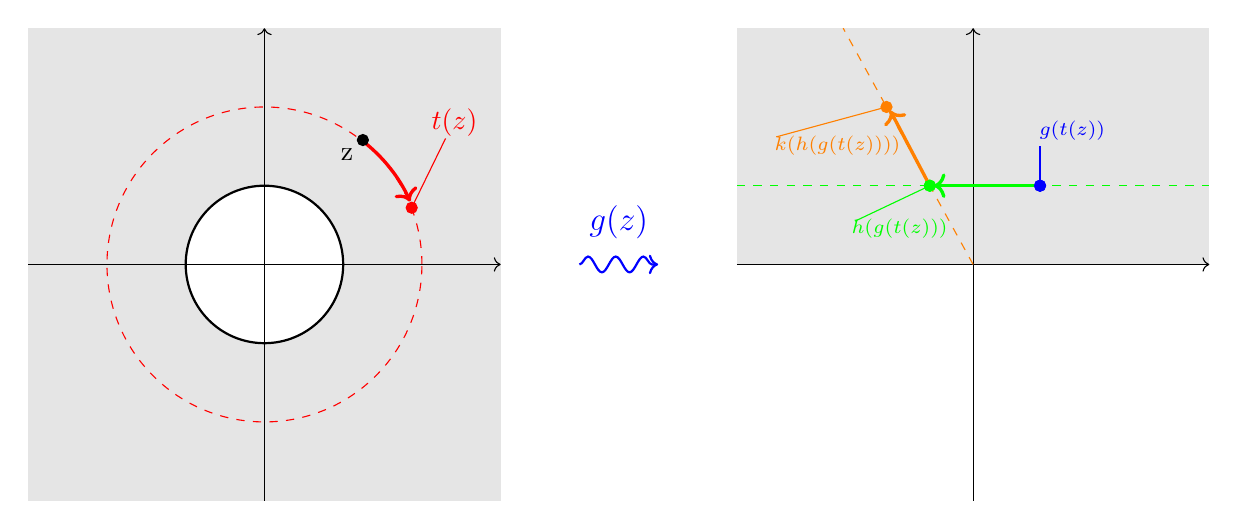
\begin{tikzpicture}

    % Plot 1: Using pgfplots for the parametric plot
    \begin{axis}[
        axis lines=none,
        trig format plots = rad,
        xmin = -3, xmax = 3,
        ymin = -3, ymax = 3,
        %domain = 0:1,
        samples=200,
        width=15cm,
        height=10cm,
        axis equal,  % Keep the aspect ratio of the plot square
        xtick=\empty, ytick=\empty  % Remove ticks for a cleaner look
    ]
        % Parametric plot for the curve
       
    \end{axis}

    % Plot 2: TikZ drawing overlaid for the exterior region of the unit disk
    \begin{scope}[shift={(0,0)}]  % Same coordinate system for overlaid drawing

        % Shade the exterior region of the unit disk
        \fill[gray!20] (-3,-3) rectangle (3,3);
        \fill[white] (0,0) circle (1);
        
        % Draw the unit circle
        \draw[thick] (0,0) circle (1);
        % Draw the larger circle of radius 2
        \draw[red, very thick, <-] (1.85,0.8) arc[start angle=24, end angle=52, radius=2];  
       
        \draw[red, dashed] (2,0) arc[start angle=0, end angle=360, radius=2];  % Arc starting at (1.5, 0.5)
        % Arc starting at (1.5, 0.5)
        % Axes
        \draw[->] (-3,0) -- (3,0);
        \draw[->] (0,-3) -- (0,3);
        
        % Add a point at (1,1.2)
        \filldraw[black] (1.25,1.58) circle (2pt);            
        % Label the point
        \node[below left] at (1.25,1.6) (z) {z};

        \node[right, red] at (2,1.8) {$t(z)$};  % Node text in red
        \filldraw[red] (1.87, 0.72) circle (2pt);            

        \draw[red, -] (2.3,1.6) -- (1.87,0.72) ;


    \end{scope}

    % Mapping arrow between two plots
    \draw[->, blue, thick, decorate, decoration={snake, amplitude=1mm}] (4,0) -- (5,0) node[blue, midway, above, yshift=0.2cm] {\large $g(z)$};

    % Plot 3: Upper half-plane
    \begin{scope}[shift={(9,0)}]
        % Shade the upper half-plane
        \fill[gray!20] (-3,0) rectangle (3,3);
        
        % Axes
        \draw[->] (-3,0) -- (3,0);
        \draw[->] (0,-3) -- (0,3);
        
        \node[below left, blue] at (1.8,1.95) (z) {\scriptsize  $g(t(z))$};
        \draw[-, blue] (0.85,1.5) -- (0.85,1);

        \filldraw[blue] (0.85,1) circle (2pt);            

        \draw[green, dashed] (-3,1) -- (3,1);
        \draw[<-, green, very thick] (-0.5,1) -- (0.85,1);
        \filldraw[green] (-0.55,1) circle (2pt);   
        
        
        \node[below left, green] at (-0.2,0.7) (z) {\scriptsize $h(g(t(z)))$};
        \draw[-, green] (-1.5,0.55) -- (-0.55,1);

        \filldraw[orange] (-1.1,2) circle (2pt);   

        \draw[-, orange, very thick, <-] (-1.05,1.95) -- (-0.55,1);

        \draw[orange, dashed] (0,0) -- (-1.65, 3);
        \filldraw[green] (-0.55,1) circle (2pt);   
        \filldraw[blue] (0.85,1) circle (2pt);            


        \node[below left, orange] at (-0.8,1.75) (z) {\scriptsize $k(h(g(t(z))))$}; 
        \draw[-, orange] (-1.1,2) -- (-2.5,1.62);

        % Label the upper half-plane
        \node at (2,1.5) {};
    \end{scope}

\end{tikzpicture}
\[\]
\noindent This plot shows us that starting with any given \(z \in \mathbb{C}\setminus \overline{D}(0;1)\) we can apply \(M(z)\) to map \(z\) to any point in the upper half plane \( \{ z \in \mathbb{C} : {Im}(z) > 0 \} \)


\[\]
\noindent \textbf{Q5.} Consider a thin membrane which minimises its internal energy on \(U = D(1;2)\) with surface height described by \(u\left(x,y\right)\) which satisfies \(u\left(x,y\right) = y^2 - x^3 \text{ on } C\left(1;2\right)\). Determine \(u\left(x,y\right)\).\newline
\linebreak
\noindent We aim to find \(g(z)\) such that \(Re(g(z)) = u(z)\) with \(u(z)|_{C(1;2)} = y^2 - x^3 \)\newline
\linebreak
\noindent Notice that on \(C(1;2)\) we have \(\left(x-1\right)^2+y^2=4\)
\[
\implies y^2 = 4 - \left(x-1\right)^2
\]
\[
    \implies y^2 = -\left(x-3\right)\left(x+1\right)
\]
Consider that if we make the ansatz:
\[
g(z) = az^3 + bz^2 + cz + d
\]
\[
\implies Re(g(z)) = Re(a\left(x+iy\right)^3 + b\left(x+iy\right)^2 + c\left(x+iy\right) + d)
\]
\[
= Re(a x^3 + i 3 a x^2 y - 3 a x y^2 - i a y^3 + b x^2 + i 2 b x y - b y^2 + c x + i c y + d)
\]
\[
=ax^3 - 3axy^2+bx^2-by^2+cx+d
\]
\(\implies\) {On } \(C(1;2)\) we have:
\[
y^2 - x^3 = ax^3 - 3axy^2+bx^2-by^2+cx+d \quad,\quad y^2 = -\left(x-3\right)\left(x+1\right)
\]
\[
\implies \left(-\left(x-3\right)\left(x+1\right)\right) - x^3 = ax^3 - 3ax\left(-\left(x-3\right)\left(x+1\right)\right)+bx^2-b\left(-\left(x-3\right)\left(x+1\right)\right)+cx+d
\]
\[
\implies -x^3 - x^2 + 2x + 3 = ax^3 -3ax\left(-x^2+2x+3\right)+bx^2-b\left(-x^2+2x+3\right)+cx + d
\]
\[
\implies -x^3 - x^2 + 2x + 3 = ax^3 +3ax^3-6ax^2-9ax+bx^2+bx^2-2bx-3b +cx + d
\]
\[
    \implies -x^3 - x^2 + 2x + 3 = 4ax^3 + x^2\left(2b-6a\right)+x\left(c-2b-9a\right)+d-3b
\]


\noindent Now equating the coefficients, we obtain:
\begin{enumerate}
    \item[\(x^3)\)] \qquad \(-1 = 4a \implies a = -\frac{1}{4} = -0.25\)
    \item[\(x^2)\)] \qquad \(-1 = 2b - 6a = 2b + \frac{3}{2} \implies b = -\frac{5}{4}= -1.25\)
    \item[\(x\,)\)] \qquad \(\,\,\,\, 2 = c-2b-9a \implies c = 2 + 2\left(-1.25\right)+9\left(-0.25\right) = -\frac{11}{4}=-2.75 \)
    \item[constant)] \qquad \(\,\,\,\, 3 = d-3b = d+3.75 \implies d = \frac{-3}{4} = -0.75\)
\end{enumerate}



\noindent Putting it all together we have:
\[
g(z) = -\frac{1}{4}z^3  -\frac{5}{4}z^2  -\frac{11}{4}z - \frac{3}{4}
\]

\[
\implies u(x,y) = Re(g(z)) =ax^3 - 3axy^2+bx^2-by^2+cx+d
\]

\[
=  -\frac{1}{4}x^3 + \frac{3}{4}xy^2 - \frac{5}{4}x^2 +\frac{5}{4}y^2 -\frac{11}{4}x - \frac{3}{4}
\]

\[
= \frac{-x^3+3xy^2-5x^2+5y^2-11x-3}{4}
\]
\[\]
\noindent Notice that because \(g\) is a polynomial in \(z\), it is holomorphic on \(\mathbb{C}\). Therefore, because \(u\) is the real part of \(g\), we have that \(u\) is harmonic. We also have shown that on \(\partial U\), our solution for \(u(x,y) = y^2 - x^3\) by the reverse of the working we used to obtain the coefficients of \(g\). Therefore it must be that \(u(x,y)\) minimises its internal energy on \(U\) as required. 
 



\hrulefill

\end{document}

